\chapter[Revisão Bibliográfica]{Revisão Bibliográfica} 
\label{cap:cap2}
%Eu acho que você quis associar o conceito de participação com governança e transparência, acho essa abordagem muito legal. 
%Mas acho que falta você trabalhar um pouco mais essa relação. Pensa que deve existir uma coerência nessa discussão:
%minha sugestão é que você desenvolva melhor o texto seguindo esse caminho: governança digital->transparência->participação

% Introdução do capítulo
Neste capítulo são apresentados os tópicos teóricos necessários para uma boa compreensão do desenvolvimento deste trabalho.

% 1a seção do capítulo 1
\section{Participação Eletrônica}
\label{sec:e-part}
Atualmente, fatores como a sociedade civil organizada sendo reconhecida pelos governos e governantes, e o consequente aumento da participação da população nos
programas governamentais, junto com a ampliação e diversificação dos temas abordados nas esferas governamentais, têm determinado um novo modelo de governança \cite{o2011government}. 
Este modelo acaba por oferecer um espaço, antes não existente,  onde o conceito de participação pode ser ampliado até o conceito de cidadania, ou seja, a participação cidadã.

\par
De acordo com a \acrshort{onu}, promover a participação cidadã é fundamental para a governança de uma sociedade civil organizada e inclusiva.
O objetivo dessa participação deve ser composto pela melhoraria do acesso às informações e aos serviços públicos,
e pelo incentivo a inclusão do cidadão nas tomadas de decisões públicas que impactem o bem estar da sociedade como um todo, e do indivíduo em particular. 
As funções de fazer política e entregar serviços públicos precisam ser reinterpretadas e os cidadãos têm que se envolver nos processos políticos \cite{bovaird2007beyond}.

\par
Sendo assim, a incorporação de novas tecnologias na relação entre estado e sociedade amplia e possibilita uma outra dinâmica a essa relação. 
Seguindo o conceito de governança digital, apresentado pela \acrshort{onu}, que trata do uso de \acrfull{tic} para atender três pilares fundamentais,
a prestação de melhores serviços pelos agentes públicos, o maior acesso a informação e a maior participação da sociedade civil em todos os ciclos de políticas públicas.
As \acrshort{tic} permitem a alavancagem desses três pilares em um alto patamar de desempenho. 

\par
A noção de governança digital é interpretada por \citeonline{reddick2012public} como o resultado da adoção de infraestruturas tecnológicas 
para a otimização da entrega de serviços à população. Ou seja, a utilização de \acrshort{tic} pelo setor público, passa a se referir ao modo como as tecnologias e a
internet podem melhorar a capacidade do Estado de formular e implementar suas políticas públicas \cite{parra2017governancca}.

\par
Deste modo, \citeonline{germani2016desafios} complementa a definição de governança digital afirmando que sua utilização pelo setor público,
deve ter o objetivo de melhorar a disponibilização de informações e o fornecimento de serviços públicos, além de incentivar o engajamento
da sociedade nos processos políticos, aprimorando os níveis de responsabilidade, transparência e efetividade do governo.

\par
A utilização de \acrshort{tic} pelo setor público tem transformado a governança global como um todo, exigindo que governos e governantes forneçam
serviços melhores, mais econômicos e eficientes às organizações e indivíduos \cite{afdb2014uneca}. 

\vspace{0.3CM}

\par
O conceito de participação eletrônica foi definido por \citeonline{macintosh2008democracy} como o uso de informações e comunicação tecnológicas a fim de ampliar e aprofundar
a participação política para que cidadãos sejam capazes de se conectar uns aos outros e aos seus representantes eleitos.
Para \citeonline{braga2016participaccao}, a possibilidade de um maior acesso as informações e ao conhecimento, permite uma maior transparência nas decisões tomadas por governantes.
\citeonline{vaz2017transformaccoes} argumenta que há a necessidade de alteração do atual modelo
\textit{broadcasting}, para um modelo mais participativo de tomada de decisões.

\par
Define-se "modelo \textit{broadcasting}" como um modelo de alocação dos recursos digitais como recursos secundários ou complementares às iniciativas presenciais
de relacionamento entre governos e sociedade. Nesse modo, são os governantes que estabelecem os momentos, formatos e conteúdo dos processos participativos e de controle social.
Isso acaba por restringir as iniciativas apenas às iniciativas governamentais, nas quais a interação e participação nas decisões e no controle social das políticas públicas 
são monopolizadas pelo Estado \cite{parra2017governancca}.

\par
Para que haja a evolução desse modelo atual, \citeonline{o2011government} sugere que o governo deve disponibilizar suas informações em uma infraestrutura que permita
a sua reutilização sistemática pela sociedade civil. Ao disponibilizar suas informação, o governo estimula o desenvolvimento de inciativas e ferramentas tecnológicas,
ampliando assim a possibilidade do uso diverso das informações \cite{zuiderwijk2012socio}.

\par
Segundo \citeonline{vaz2017transformaccoes}, o crescimento do conceito e da comunidade \textit{open source}, atrelados ao compartilhamento de dados governamentais,
permite a produção descentralizada de aplicações, serviços e sistemas tecnológicos. Criando assim, o que o autor chama de "segunda geração de governança digital", 
que consiste na busca por iniciativas além das unidirecionais(\textit{broadcasting}) , onde o governo apenas disponibiliza os dados captados sobre a população.

\par
O conceito de governança digital \textit{open source} democratiza a tomada de decisão e incentiva a colaboração voluntária entre os indivíduos \cite{rushkoff2003open}.
Diversos paradigmas, sobre este modelo de tomada de decisão, vêm sendo reexaminados, e o papel do gestor público e do cidadão têm sido reavaliados.
O uso das ferramentas de participação eletrônica tem se disseminado para diversos casos de uso e em muitos ambientes diferentes \cite{medeiros2009novos}.

%!!!!!!!!!!!!!!!!!!!!!!!!!!!!!!!!!!!!!!!!!

OS PROXIMOS 3 PARAGRAFOS FICAM NESSA SESSÃO?

%!!!!!!!!!!!!!!!!!!!!!!!!!!!!!!!!!!!!!!!!!

\par
São muito os exemplos de ferramentas de participação eletrônica, contudo, a sociedade civil ainda não têm se engajado plenamente ao uso de todos os modelos ferramentas.
Para exemplificar, temas de grande interesse popular como as reformas trabalhista, tributária e da previdência social brasileira, recebem grande atenção dos 
veículos de comunicação, são diversas vezes citadas propostas de governantes pleiteando cargos e são relatadas por especialistas como fundamentais para o desenvolvimento do país.
Seguindo o raciocínio, espera-se um engajamento relativamente grande perante esses assuntos, porém, a ferramenta de participação eletrônica Wikilegis, desenvolvida pela câmara
dos deputados do Brasil, que disponibiliza um ambiente onde a sociedade civil pode analisar os projetos de leis e contribuir com sugestões
de nova redação a artigos ou parágrafos, que serão acompanhadas pelos relatores das proposições, conta com números pífios de sugestões para os projetos de reformas.
São 221 sugestões para a reforma da previdência, 129 sugestões para a reforma tributária e míseras 50 sugestões para a reforma trabalhista. 
Os números mostram a dificuldade de engajar a sociedade civil em assuntos políticos mais complexos e que demandam tempo e estudo.

\par
Por outro lado, o site Votanaweb conta com um painel onde são mostrados projetos de leis, seus propositores e componentes gráficos para representar a votação dos cidadãos.
Assim, o cidadão pode comparar sua intenção de voto com as dos demais cidadãos e com os votos efetivados pelos representantes, além de contar com a descrição dos votos por gênero, 
região e idade. Os projetos têm em média sete mil votos, onde o mais votado conta com certa de quase quinze mil votos. 

\par
Isso indica que o engajamento da sociedade civil tem muito espaço para crescer \cite{o2011government}, fica o desafio aos atores da sociedade, governantes, empresas e indivíduos,
à criação de ferramentas de participação eletrônica que estimulem o engajamento do cidadão.

\section{Ferramentas de Participação Eletrônica}
\label{sec:e-part tools}
Devido aos incentivos gerados por esses novos paradigmas de tomada de decisão, muitas ferramentas de participação eletrônica têm sido desenvolvidas focadas nesse escopo.
Essas ferramentas podem ter aplicações direcionadas a cidades, bairros, regiões, estados e/ou países. 

%!!!!!!!!!!!!!!!!!!!!!!!!!!!!!!!!!!!!!!!!!!!!!!!!!!!!!!!!!!!!!!!

 ====> Descrever os 29 itens de classificação?!

%!!!!!!!!!!!!!!!!!!!!!!!!!!!!!!!!!!!!!!!!!!!!!!!!!!!!!!!!!!!!!!!

Alguns exemplos podem ser encontrado na Tabela \ref{tab:ferramentas}.

\begin{table}[!ht]
    \centering
    \caption{Ferramentas de Participação Eletrônica}
    \label{tab:ferramentas}
    \begin{tabular}{l*{2}{>{\raggedright\arraybackslash}p{0.5\linewidth}}}
    \toprule
        Nome                             & Acesso                           \\ 
    \midrule
        Crowd For Roads                  & c4rs.eu                          \\
        Decidim Barcelona                & decidim.barcelona                \\
        e-Cidadania                      & senado.leg.br/ecidadania         \\
        Iniciativa de Cidadania Europeia & ec.europa.eu/citizens-initiative \\
        LabRIO                           & lab.rio                          \\
        Mandato Participativo            & saopaulo.sp.leg.br               \\
        Participa.BR                     & participa.br                     \\
        Patio                            & patiolla.fi                      \\
        Plataforma Brasil                & plataformabrasil.org.br          \\
        Portal e-Democracia              & edemocracia.camara.gov.br        \\
        SigaLei                          & sigalei.com.br                   \\
        Visor Urbano                     & visorurbano.com                  \\
        Vote na Web                      & votenaweb.com.br                 \\ 
        We The People                    & petitions.whitehouse.gov         \\
        WeLive                           & welive.eu                        \\
    \bottomrule
    \end{tabular}
\end{table}

\newpage

As novas tecnologias mostraram uma gama de possibilidades para que os cidadãos ampliem o peso de sua participação nas decisões políticas,
melhorando a capacidade de mobilização, articulação, e possibilitando um maior envolvimento dos atores sociais \cite{araujo2015democracia}.\\

\par
\citeonline{saebo2008shape} dividem os atores sociais em quatro grupos: 

\begin{minipage}{.66\textwidth}	
   \textit{I}) Cidadãos, \\
   \textit{II}) Governantes, \\
   \textit{III}) Instituições estatais e \\
   \textit{IV}) Instituições Voluntárias. \\
\end{minipage}

\par
Esse agrupamento feito pelo autor supracitado é uma abstração da análise de \citeonline{macintosh2006evaluating}, deixando de lado um quinto grupo:

\par
\textit{V}) Provedores de Tecnologia.

\par
Contudo, \citeonline{wimmer2007ontology} agrupa esses atores mais objetivamente, dividindo-os em apenas dois grupos, são eles:\\

\begin{minipage}{.75\textwidth}	
   \textit{a}) Beneficitários da utilização das ferramentas e \\
   \textit{b}) Responsáveis pela administração da ferramenta de participação.  \\
\end{minipage}

Esses grupos começaram a se utilizar de ferramentas de participação eletrônica, muitas vezes em projetos pilotos,
sem estratégias para medir os impactos gerados, as análises de performance ou as respostas dos cidadãos beneficiados \cite{macintosh2008democracy}.
Muitos autores chamam atenção para fato das ferramentas de participação serem predecessoras dos modelos de escolha e classificação para elas 
\cite{millard2006egovernance,macintosh2008democracy,reddick2012public}.

\par
A \acrfull{ocde}, juntamente com a \acrshort{onu} e a \acrfull{ue} criaram \textit{frameworks} para a avaliação das ferramentas através de indicadores. 
Atualmente, governantes podem encontrar diretrizes para seguir na hora de desenvolver uma atividade de participação eletrônica.

%==================================================================================================================================================================================================
\newpage
\section{Taxonomia}
\label{sec:taxonomia}
Com o objetivo de apresentar um panorama conceitual sobre o termo taxonomia e contextualizar o assunto, \citeonline{novo2007elaboraccao} diz:

\hspace{4cm}
\begin{minipage}{.66\textwidth}		
    \begin{singlespace}
        \fontsize{10}{12}\selectfont O conceito de taxonomia não emerge de repente como uma fórmula para solucionar problemas de representar o conhecimento de um dado domínio.
        É resultado de um longo processo histórico que se estendeu através de estudos e investigações que culminaram numa construção teórica.
        Esta evolução não foi linear tampouco ocorreu em um mesmo momento histórico, pois um único modelo não conseguiria responder de imediato a questões tão particulares 
        e complexas encontradas nas diversas áreas do conhecimento.
        \end{singlespace}
\end{minipage}
\vspace{0.3CM}

Taxonomia é, por definição, classificação, sistemática. Tradicionalmente utilizada para a classificação das espécies em botânica e zoologia, adotando uma definição binária.
\par
A utilização de taxonomia nos sistemas de informação não leva em consideração família, gênero ou espécie, mas sim conceitos.
As classes e subclasses de uma taxonomia se apresentam de maneira lógica, suportada por princípios classificatórios.\cite{campos2012taxonomia}
\par
Um dos recursos fundamentais para a gestão da informação e do conhecimento é o desenvolvimento de taxonomias \cite{dal2015ferramentas}.
\citeonline{aganette2010elementos} diz que diferente do princípio dicotômico adotado na taxonomia dos seres vivos, atualmente, faz-se possível a construção de taxonomias
policotômicas, ou seja, onde um objeto é classificado em tantas classes, e subclasses quantas necessárias, dentro um domínio especializado.
\par
Sendo assim, é possível utilizar a representação taxonômica da Figura \ref{fig:exemploTaxonomia} para classificar um objeto, arbitrariamente escolhido,
de acordo com os nós F e C, por exemplo.

\begin{figure}[!ht]
\begin{tikzpicture}[level 1/.style={sibling distance=5cm},level 2/.style={sibling distance=2.5cm}]
    \node {T}
        child { node {A}
        child {node{D}}
        child {node{E}}
        child {node{F}}
        child {node{G}}
        child {node{H}}
        }
        child { node {B}}   
        child { node {C}}  
    ;
\end{tikzpicture}
\caption{Exemplo de Taxonomia}
\label{fig:exemploTaxonomia}  
\end{figure}

%==================================================================================================================================================================================================
\subsection{Taxonomia para Ferramentas de Participação Eletrônica}
\label{subsec:taxonomia e-part tools}
\par
Por ser tratar de um assunto específico, inovador e relativamente novo, durante pesquisa para elaboração deste trabalho,
o único exemplo de taxonomia para ferramentas de participação eletrônica encontrado foi o esquema taxonômico elaborado pelos participantes do projeto de pesquisa Vispública, 
que será abordado na Seção \ref{subsec:taxonomiaElaborada}

%==================================================================================================================================================================================================
%\subsection{Taxonomia para Outras Ferramentas}
%\label{subsec:taxonomia other tools}

%==================================================================================================================================================================================================
\subsection{Taxonomia para Outras Áreas da Computação}
\label{subsec:taxonomia other computer areas}
Taxonomia, no contexto da computação, tem aplicação em distintas áreas. A utilização de estruturas taxonômicas para classificar sistemas, arquiteturas e arquivos data de mais de
cinquenta anos. Uma das classificações taxonômica com maior relevância para a área da computação é a chamada "Taxonomia de Flynn",
onde \citeonline{flynn1966very} classificou as arquiteturas de computadores da seguinte forma:\\

\begin{minipage}{.66\textwidth}
    \begin{singlespace}
        \begin{itemize}
            \item \acrfull{sisd}
            \item \acrfull{simd}
            \item \acrfull{misd}
            \item \acrfull{mimd}
        \end{itemize}
    \end{singlespace}
\end{minipage}
\vspace{0.5cm}

\begin{figure}[!ht]
    \begin{tikzpicture}[level 1/.style={sibling distance=5cm},level 2/.style={sibling distance=2.5cm}]
        \node {T}
            child { node {\acrshort{sisd}}}   
            child { node {\acrshort{simd}}}  
            child { node {\acrshort{misd}}}   
            child { node {\acrshort{mimd}}}  
        ;
    \end{tikzpicture}
    \caption{Taxonomia de Flynn}
    \label{fig:taxonomiaFlynn}  
\end{figure}

\vspace{0.5cm}
\par
A área de tolerância a faltas, da engenharia de \textit{software}, tem taxonomias comumente adotadas para definir termos e técnicas.
Entre as mais conhecidas estão a taxonomia proposta por \citeonline{gartner1999fundamentals}, abordando diversos conceitos e os aplicando a um cenário distribuído,
e a taxonomia apresentada por \citeonline{avizienis2004basic}, definindo conceitos sobre tolerância a faltas e segurança computacional.

\par
\citeonline{sondhi2018taxonomy} criou uma taxonomia que pode ser usada para prever as ações ou intenções de um usuário em particular de uma dada loja virtual
e então personalizar o algoritmo de busca para indicar as necessidades específicas desse usuário.

\par
Vale ressaltar a grande utilização de taxonomia por lojas virtuais, e o grande número de trabalhos encontrados sobre taxonomia aplicada a esse setor.

%==================================================================================================================================================================================================
\subsection{Taxonomia Elaborada}
\label{subsec:taxonomiaElaborada}
\par
Por meio do projeto Vispública foi elaborada a taxonomia mostrada na Figura \ref{fig:taxonomia-vispublica}. Neste trabalho, o esforço foi no sentido de fornecer a classificação de
ferramentas de participação através de uma taxonomia, de forma que seja possível associar uma ferramenta às dimensões propostas e também permitir uma compreensão
geral do que existe acerca das iniciativas de e-participação identificadas na literatura.

\begin{figure}[!ht]
    \centering
    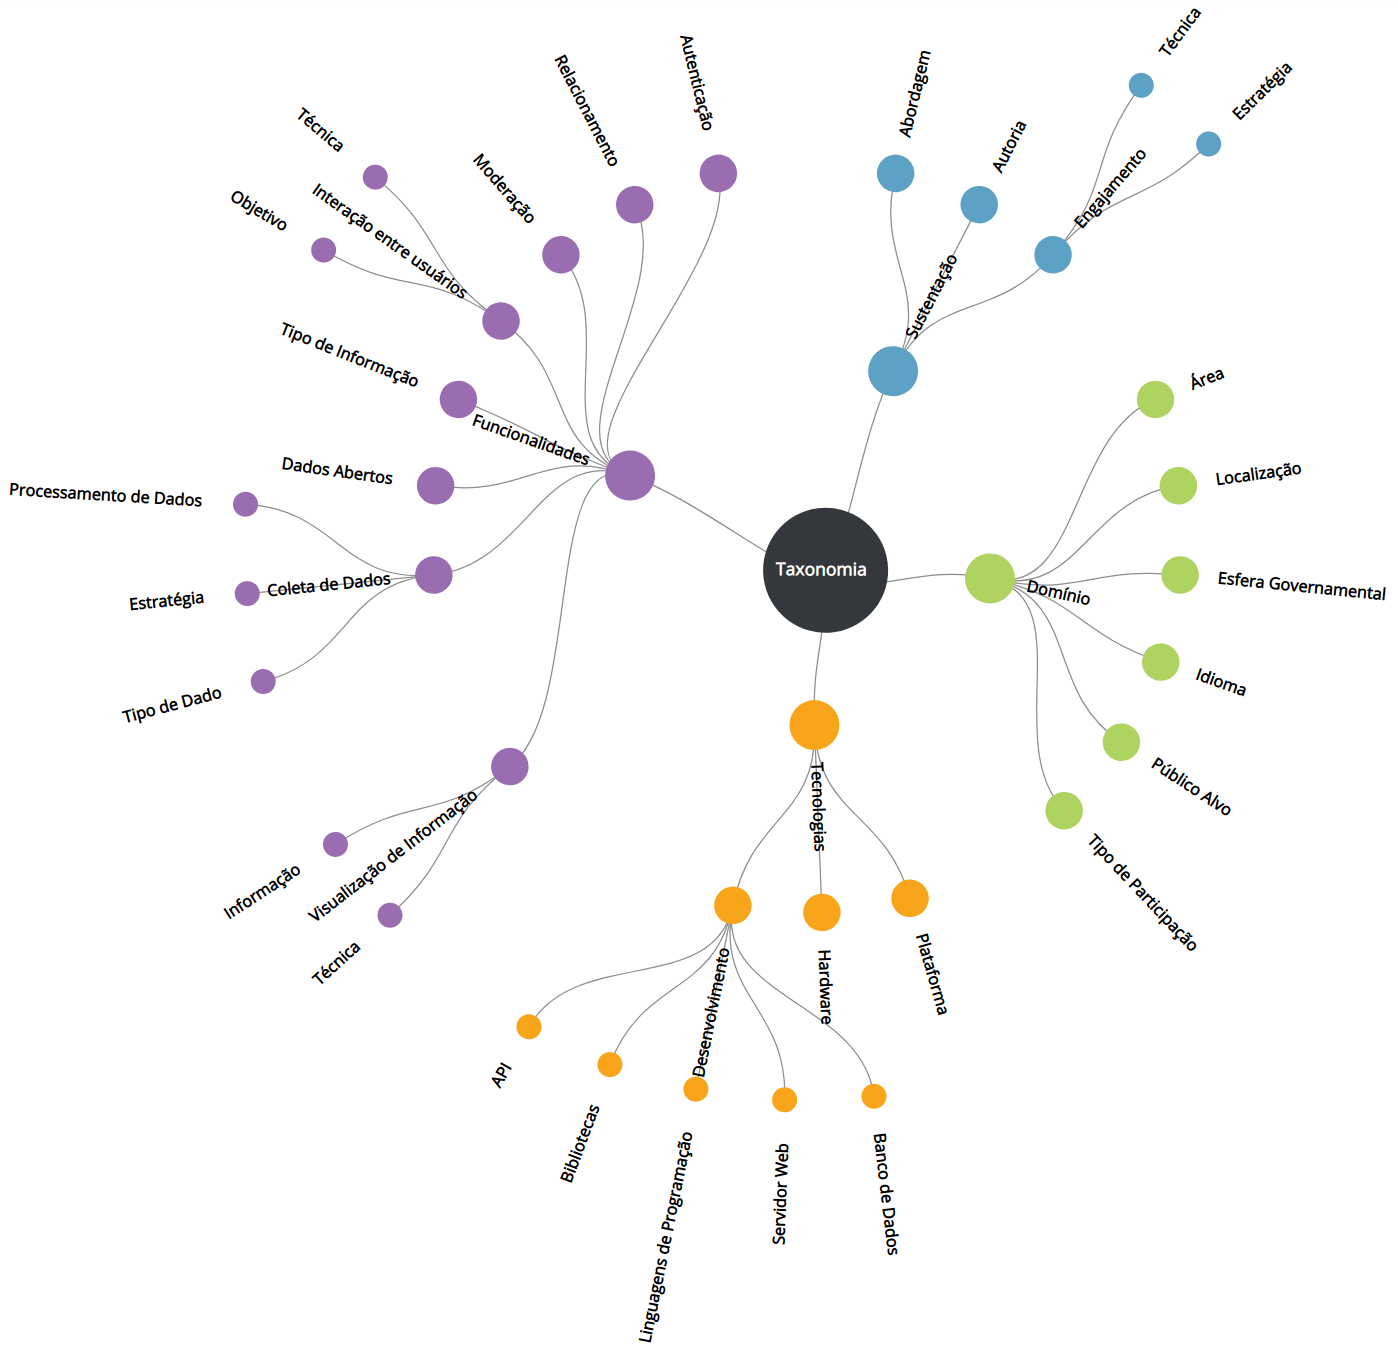
\includegraphics[scale=0.3]{./figuras/taxonomia-cropped.png}
    \caption{Taxonomia elaborada pelo projeto Vispública}
    \label{fig:taxonomia-vispublica}
\end{figure}

